\chapter{Conclusions and perspectives}\label{ch:conclusions}

This Thesis presented the measurement of the \pt-differential strange over non-strange \ds/\dpl production-yield ratio in proton-proton collisions at \thirteen, performed with the upgraded ALICE detector and the data collected during the LHC Run~3 data-taking period. 

The analysis was performed via the full reconstruction of displaced decay topologies through the same hadronic decay channel $\ds, \dpl \rightarrow \phi\pi^+\rightarrow\mathrm{K^+K^-\pi^+}$. Multiclass Machine Learning models using the XGBoost algorithm were employed to enhance the selection efficiency of the signal candidates and to reduce the combinatorial background. Additionally, they were used to increase the relative contribution of prompt \ds and \dpl mesons (i.e., those directly produced in the hadronisation of a charm quark or through the strong decay of a directly produced excited charm-hadron or charmonium state) in the selected sample. The measurement was carried out in 14 transverse-momentum intervals in the range $0.5<\pt<24$~\gevc, and extended the \pt coverage at low \pt with respect to previous measurements performed by the ALICE Collaboration at $\sqs = 5.02, 7$ and $13$~\tev, reported in Refs.~\cite{ALICE:2021mgk,ALICE:2017olh,ALICE:2023sgl}, respectively. Additionally, thanks to the larger data sample collected during the LHC Run~3 data-taking period, and the reconstruction of both D-meson species in the same decay channel, the results presented in this Thesis significantly reduced both the statistical and systematic uncertainties of the measurement, and improved its granularity with respect to the measurements performed by both the ALICE and LHCb~\cite{LHCb:2015swx} Collaborations at mid and forward rapidities, respectively.

The measurements performed at midrapidity ($\lvert y\rvert<0.5$) at the centre-of-mass energies of  $\sqs = 5.02, 7, 13$ and \thirteen by the ALICE Collaboration indicate no significant energy-dependence of the \ds/\dpl production-yield ratio. Furthermore, the comparison of the results presented in this Thesis, performed at midrapidity ($\lvert y\rvert<0.5$) at \thirteen with the ALICE experimental apparatus, with those obtained by the LHCb Collaboration at forward rapidity in the $2.0<y<4.5$ at $\sqs=13$~\tev, shows a good agreement within the uncertainties. This indicates no significant dependence of the \ds/\dpl ratio on the studied rapidity. 

This measurement provides state-of-the-art results for the understanding of the hadronisation mechanisms (i.e., the transition from colour-charged partons (quarks and gluons) produced in a collision into colour-neutral hadrons) of charm quarks in high-energy hadronic collisions. As described in Chapter~\ref{ch:openHF}, the hadronisation mechanism is expected to be modified in the presence of a deconfined medium, the Quark-Gluon Plasma (QGP), which is formed in high-energy nuclear collisions. In a thermalised deconfined medium, charmed hadrons can be produced through coalescence of charm quarks, which are produced before the QGP is formed, with light quarks from the medium. Additionally, in the presence of a QGP, the production of strange quarks is expected to be enhanced, as the high temperatures reached in the medium allow for the thermal production of strange-antistrange quark pairs. The measurement of the \ds/\dpl production-yield ratio is a powerful tool to investigate the hadronisation mechanisms of charm quarks, and is a sensitive probe to the phenomenon of strangeness enhancement. 

Several measurements confirmed the production of the QGP in high-energy nuclear collisions, such as Refs.~\cite{NA50:1997hlx,WA97:2000apo,ALICE:2018vuu}. The production of an extended QGP phase is not expected in proton-proton collisions, as the system size is too small to reach the critical energy density required for QGP formation. However, recent measurements performed at the LHC~\cite{CMS:2016fnw,CMS:2010ifv,ALICE:2019zfl} provide evidence for the presence of collective effects in small systems, such as proton-proton and proton-lead collisions, which are usually associated with the formation of a QGP. The ALICE Collaboration reported the observation of a smooth increase in the strange- and multi-strange-hadron production with the charged-particle multiplicity in proton-proton collisions at $\sqs=7$~\tev~\cite{ALICE:2016fzo}, reaching, for the highest multiplicity classes, values compatible with those measured in the most central lead-lead collisions. 

\begin{figure}[tb]
    \centering
    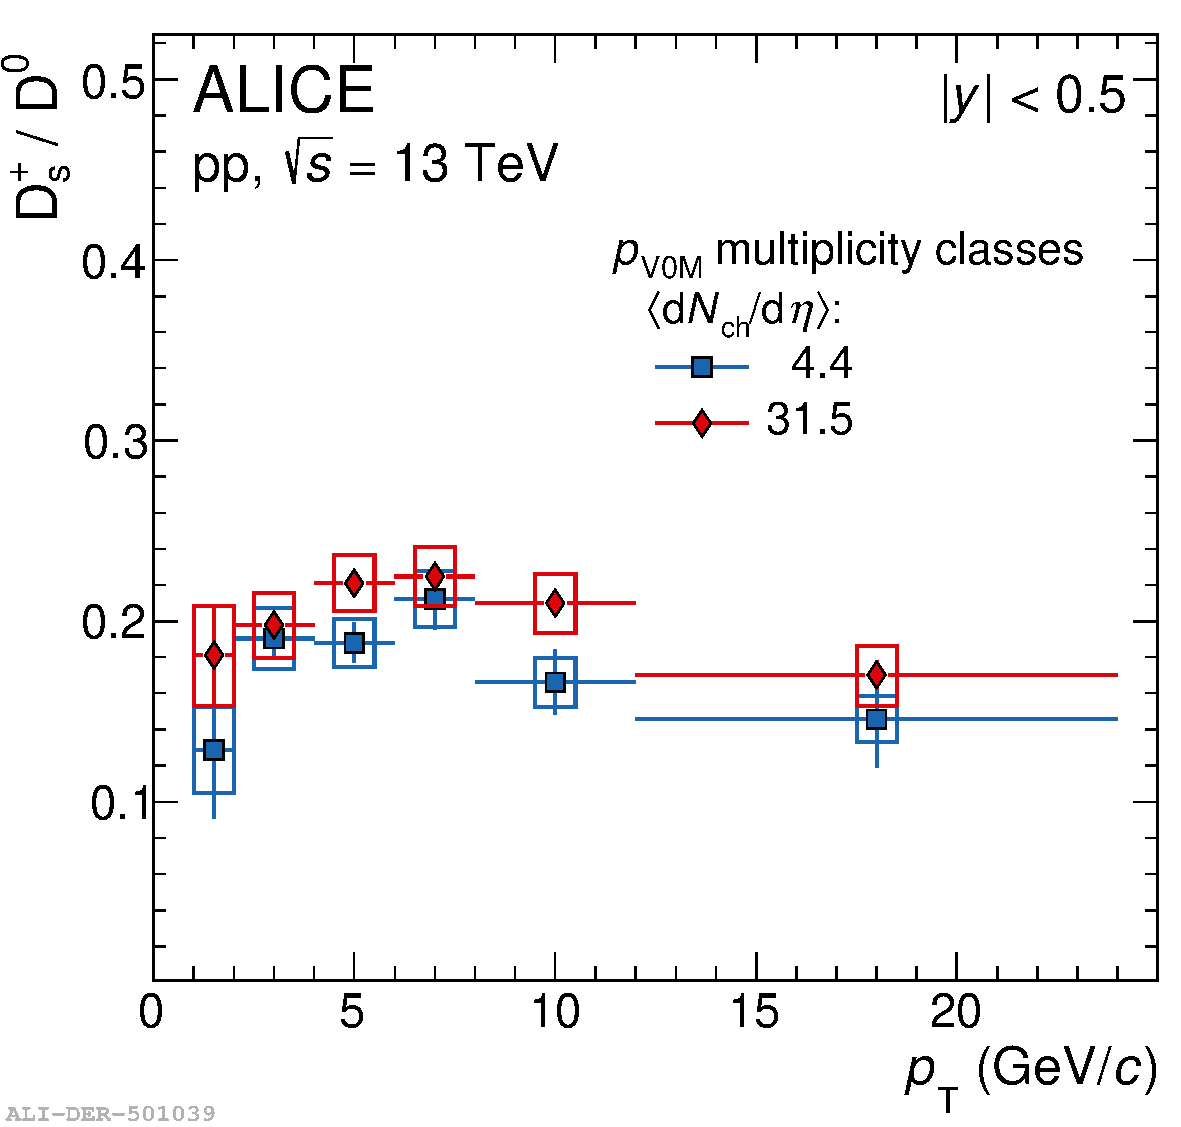
\includegraphics[width=0.7\textwidth]{Figures/Chapter 9/DsD0Ratios_LowHighMult_V0M_Derived.pdf}
    \caption{Strange over non-strange \ds/\dz production-yield ratio as a function of \pt for two different multiplicity classes measured at midrapidity ($\lvert y\rvert<0.5$) in proton-proton collisions at $\sqs=13$~\tev by the ALICE Collaboration~\cite{ALICE:2021npz}. Figure taken from the ALICE figure repository~\cite{ALICE_figures}.}
    \label{fig:ALICE_DsD0VsMultiplicity}
\end{figure}

Previous measurements of the multiplicity-dependence of the strange over non-strange \ds/\dz production-yield ratio performed at midrapidity ($\lvert y\rvert<0.5$) by the ALICE Collaboration~\cite{ALICE:2021npz} did not provide a clear indication of the strangeness enhancement in proton-proton collisions at $\sqs=13$~\tev. The results are illustrated in Fig.~\ref{fig:ALICE_DsD0VsMultiplicity}, where the measured \ds/\dz production-yield ratio is shown as a function of \pt for two different multiplicity classes. The results show a slight increase of the \ds/\dz production-yield ratio with the charged-particle multiplicity, although the two \pt-differential measurements are compatible within their uncertainties. The methodologies and results presented in this Thesis provide a solid foundation for future studies of the strangeness enhancement in the heavy-flavour sector. The strategy of using the \dpl meson as a reference for the non-strange production, as well as the reconstruction of both \ds and \dpl mesons in the same hadronic decay channel allows for a significant reduction of the systematic uncertainties of the measurement. The measurement of the multiplicity dependence of the \ds/\dpl production-yield ratio may provide more precise results than those achieved through the usage of the \dz meson as a reference for non-strange D meson production, and, thereby, provide a more sensitive probe to the phenomenon of strangeness enhancement in proton-proton collisions. Additionally, the much larger data sample collected during the LHC Run~3 data-taking period will allow for the extension of the measurement to lower \pt values, where the effects of the strangeness enhancement are expected to be more pronounced, increase the statistical precision of the results, and perform a more \pt- and multiplicity-differential measurement.

%\begin{figure}[tb]
%    \centering
%    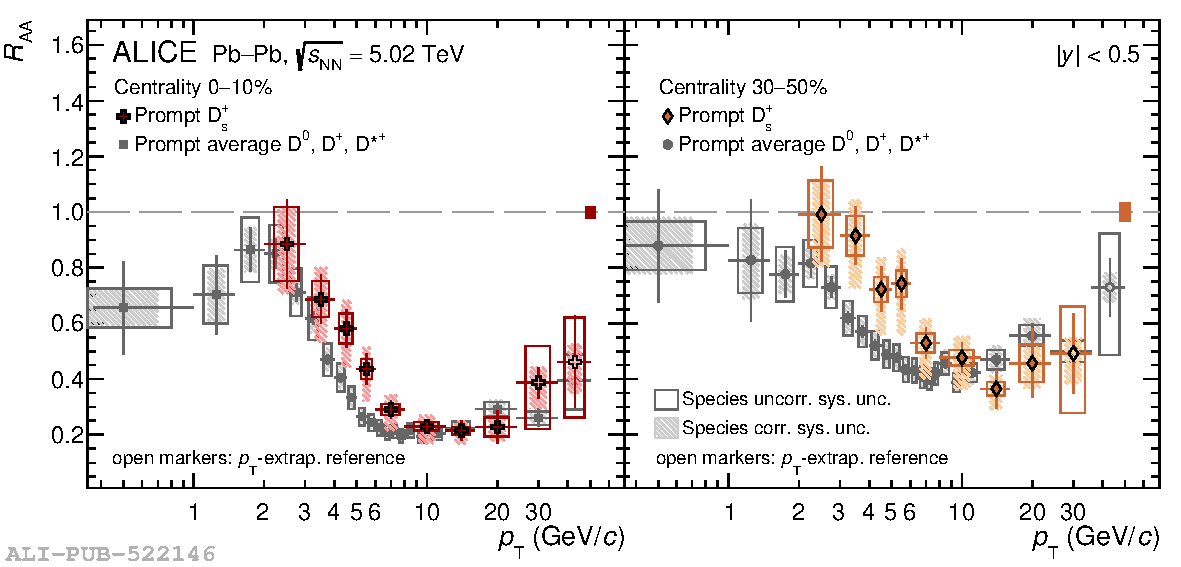
\includegraphics[width=\textwidth]{Figures/Chapter 9/PromptDs_vs_PromptD_Raa_2pads_1.pdf}
%    \caption{\raa of prompt \ds meson and average \raa of prompt \dz, \dpl, and $\mathrm{D^{*+}}$ mesons %as a function of \pt for the 0--10\% (left panel) and 30--50\% (right panel) centrality classes %measured at midrapidity ($\lvert y\rvert<0.5$) in Pb--Pb collisions at \mbox{$\snn=5.02$~\tev} by the %ALICE Collaboration~\cite{ALICE:2021npz}.}
%    \label{fig:RAA_Ds}
%\end{figure}

\begin{sloppypar}
The multiplicity phase space can be further explored by measuring the strange over non-strange D meson production-yield ratio in Pb--Pb collision, where much higher charged-particle multiplicities are reached. Previous measurements performed by the ALICE experiment at a centre-of-mass energy per nucleon pair of \mbox{$\snn=5.02$~\tev~\cite{ALICE:2021kfc}} did not provide a clear indication for the phenomenon of strangeness enhancement. %Figure~\ref{fig:RAA_Ds} shows the nuclear modification factor \raa of prompt \ds mesons, compared to the average \raa of prompt \dz, \dpl, and $\mathrm{D^{*+}}$ mesons, as a function of \pt. Results from the 0--10\% and 30--50\% centrality classes are shown in the left and right panels, respectively. The measured \raa of prompt \ds mesons in Pb--Pb collisions is compatible within uncertainties with that of other non-strange D mesons for $\pt\gtrsim10$\gevc, where the hadronisation process is expected to occur mainly via fragmentation. At lower \pt, where the coalescence mechanism is expected to play a more relevant role, the measured \raa of prompt \ds mesons is systematically higher than that of non-strange D mesons, although the results are compatible within one standard deviation for both central and semicentral collisions.
\end{sloppypar}


\begin{figure}[htb]
    \centering
    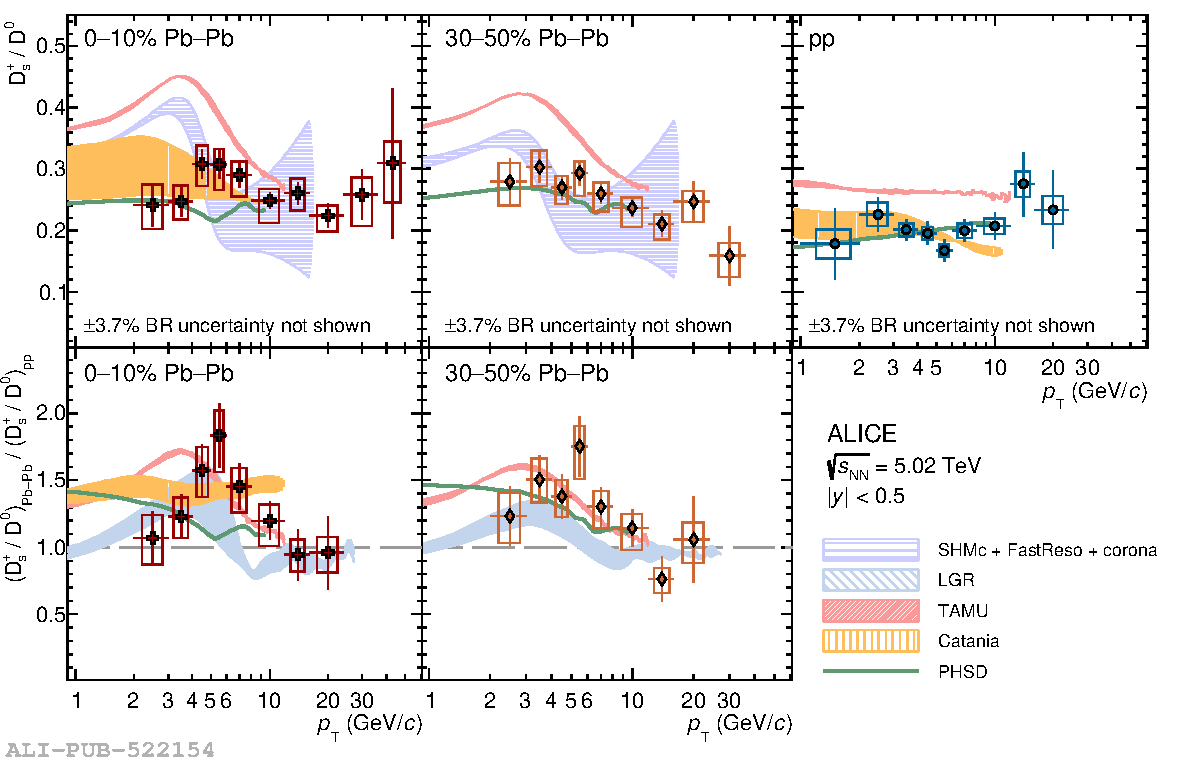
\includegraphics[width=\textwidth]{Figures/Chapter 9/Ratio_and_DoubleRatio_DsOverD0_PbPb_pp_5TeV_vs_models_1.pdf}
    \caption{Top panels: \ds/\dz \pt-differential production-yield ratios in the 0--10\% (left panel) and 30--50\% (middle panel) centrality intervals measured in Pb--Pb collisions at \mbox{$\snn=5.02$~\tev} by the ALICE Collaboration and in pp collisions (right panel) at the same centre-of-mass energy measured by the ALICE Collaboration, compared with theoretical calculations based on charm-quark transport in a hydrodynamically expanding QGP and statistical hadronisation. Bottom panels: \ds/\dz \pt-differential ratios in Pb--Pb collisions divided by those in pp collisions, in the 0--10\% (left panel) and 30--50\% (right panel) centrality intervals, compared with theoretical calculations. Figure taken from Ref.~\cite{ALICE:2021npz}.}
    \label{fig:Double_ratio}
\end{figure}

The results from the measurement of the double ratio of strange over non-strange D meson production-yield ratios in Pb--Pb collisions compared to pp collisions are shown in Fig.~\ref{fig:Double_ratio}. In the top row, the \pt-differential \ds/\dz production-yield ratios in the 0--10\% and 30--50\% centrality classes measured in Pb--Pb collisions at \mbox{$\snn=5.02$~\tev} by the ALICE Collaboration, and in pp collisions at the same centre-of-mass energy are shown. The results are compared with theoretical calculations based on charm-quark transport in a hydrodynamically expanding QGP and statistical hadronisation. The Catania model~\cite{Plumari:2017ntm,Scardina:2017ipo}, already introduced in Chapter~\ref{ch:openHF} for pp collisions, implements the coalescence mechanism in Pb--Pb collisions through the Wigner formalism~\cite{Dover:1991zn} at the phase boundary, and describes the \ds/\dz production-yield ratio in pp and central Pb--Pb collisions. In the TAMU~\cite{He:2014cla} model, a combined recombination and fragmentation approach is implemented. The former is realized via the Resonance Recombination Model (RRM)~\cite{Ravagli:2007xx} where the recombination probability for the two-body case is controlled by resonance amplitudes and is expressed as a relativistic Breit-Wigner cross-section. It significantly overestimates the measured \ds/\dz ratio by a similar amount in the two colliding systems. In the Parton-Hadron-String Dynamics (PHSD) model~\cite{Song:2015sfa} a kinetic approach is applied, and the hadronisation in heavy-ion collisions is described via a Monte Carlo simulation of the coalescence process in competition to fragmentation. It describes the \ds/\dz production-yield ratio in central and semicentral Pb--Pb collisions and pp collisions within uncertainties. Lastly, the GSI-Heidelberg Statistical Hadronisation Model~\cite{Andronic:2021erx} (SHMc), is reported for central and semicentral Pb--Pb collisions. In this model, the \pt spectra of charm hadrons are modelled with a core-corona approach. In the low-\pt region, the charm production is dominated by the core contribution, described with a Blast Wave function. The corona contribution is parametrised from measurements in pp collisions and is relevant at high \pt. The \pt-spectra modification due to resonance decays is computed using the FastReso package~\cite{Mazeliauskas:2018irt}. It provides a similar \pt shape for the \ds/\dz production-yield ratio as that provided by the TAMU model.


In the bottom row, the ratio between the \ds/\dz production-yield ratios in Pb--Pb collisions and those in pp collisions is shown for the 0--10\% and 30--50\% centrality classes. The average values of the double ratio in the $2 < \pt < 8$~\gevc interval are larger than unity by about $2.3\sigma$ and $2.4\sigma$ of the combined statistical and systematic uncertainties, for the 0--10\% and 30--50\% centrality intervals, respectively. It is compared with predictions from the TAMU and Langevin-transport with Gluon Radiation (LGR) models~\cite{Li:2019lex} (which implements the coalescence mechanism at the phase boundary), which predict a peak at $\pt\sim3-4$~\gevc. This peak could be attributed to the different masses of the \ds and \dz mesons and the collective radial expansion of the system, which provides an equal velocity boost to all particles. A similar \pt shape is predicted by the GSI-Heidelberg SHMc model. The Catania and PHSD models predict an almost flat \pt dependence of the double ratio, with a mild decreasing trend with \pt from the latter. 


The results discussed above do not allow for drawing firm conclusions on the phenomenon of strangeness enhancement in Pb--Pb collisions given the large uncertainties. Additionally, the studied centrality classes do not provide a complete picture of a possible trend in the production of strange hadrons as a function of the centrality of the collision (which, in turn, provides information on the partonic densities reached in the formed medium). A more comprehensive study would allow to also probe both the intermediate centrality (10--30\%) and the most peripheral collisions (50--100\%), which could not be explored during the LHC Run~2 data-takin period because of the limited data available.

The double ratio of \ds/\dpl production-yield ratios in Pb--Pb and pp collisions, will provide a clearer picture of the phenomenon of strangeness enhancement. It would doubly benefit from the reduction of the systematic uncertainties from the reconstruction of both D mesons in the same decay channel, as the improvement would affect both the numerator (results in Pb--Pb collisions) and the denominator (results in pp collisions) of the double ratio. Additionally, the statistical uncertainties of the measurement will be significantly reduced thanks to the larger data sample collected during the LHC Run~3 data-taking period. This will allow the extension of the measurement to lower \pt values, where the effects of the strangeness enhancement are expected to be more pronounced, due to the onset of the coalescence hadronisation mechanism, and to explore the whole centrality phase space, from the most central (where the largest deconfined mediums are formed) to the most peripheral collisions (where the effects of the QGP are expected to be less pronounced). With these perspectives, the ALICE Collaboration will provide a state-of-the-art measurement of the strangeness enhancement in the heavy-flavour sector, with a comprehensive study of the hadronisation mechanisms of charm quarks in high-energy nuclear collisions, from the lowest multiplicities reached in pp collisions to the highest multiplicities reached in Pb--Pb collisions.

In the next Chapter, a first study of the reconstruction of the \ds and \dpl mesons using the data from Pb--Pb collisions collected during the 2023 data-taking period will be presented. The results will provide a first insight into the performance of the analysis strategy presented in this Thesis in the heavy-ion environment.



